%----------------------------------------------------------------------------------------
%	HOMEWORK ASSIGNMENT EE8744
%----------------------------------------------------------------------------------------

%----------------------------------------------------------------------------------------
%	PROLOUGE 
%----------------------------------------------------------------------------------------
\documentclass[a4paper, 11pt]{article}
\usepackage[scale=0.85]{geometry} 		% Reduce document margins
\usepackage{hyperref} 					% Required for hyperlinks i.e. e-mail %
\usepackage{titlesec} 					% Used to customize the \section command
\usepackage[T1]{fontenc}				% Used to have both Bold and Small caps in heading
\usepackage{amsmath}					% Used to write equations
\usepackage{amssymb}					% Used to write math symbols e.g. R = real number set
\usepackage{autobreak}
\usepackage{graphicx}					% Used to include images
\usepackage{tabularx} 					% For custom table %
\usepackage{mathtools}					% For define notation
\usepackage{bbm}
\allowdisplaybreaks
%----------------------------------------------------------------------------------------
%	CUSTOM MACRO DEFINITION AND ENVIRONMENT MODIFICATION
%----------------------------------------------------------------------------------------
\titleformat{\section}{\bfseries\Large\scshape\filcenter}{}{0em}{}[{\titlerule[1pt]}] % Text formatting of sections
\titlespacing{\section}{0pt}{3pt}{3pt} % Spacing around sections
\pagestyle{empty} % Removes page numbering
\newcommand{\xVec}{\ensuremath{\boldsymbol{x}}}
\newcommand{\wVec}{\ensuremath{\boldsymbol{w}}}
\newcommand{\muVec}{\ensuremath{\boldsymbol{\mu}}}
\newcommand{\mVec}{\ensuremath{\boldsymbol{m}}}
\newcommand{\sVec}{\ensuremath{\boldsymbol{S}}}
\newcommand{\sigmaVec}{\ensuremath{\boldsymbol{\sigma}}}
\newcommand{\SigmaVec}{\ensuremath{\boldsymbol{\Sigma}}}
\DeclareMathOperator*{\minimize}{minimize}
%----------------------------------------------------------------------------------------
%	MAIN BODY
%----------------------------------------------------------------------------------------
\begin{document}
	%----------------------------------------------------------------------------------------
%	HEADER
%----------------------------------------------------------------------------------------
\section{HW 3}
\begin{tabularx}{\textwidth}{l}
	\hspace*{-0.8cm}\large\textsc{Arnab Dey}\\
	\hspace*{-0.8cm}Student ID: 5563169\\
	\hspace*{-0.8cm}Email: dey00011@umn.edu\\
\end{tabularx}
\bigskip
\par
    %----------------------------------------------------------------------------------------
%	SOLUTION 1
%----------------------------------------------------------------------------------------
\subsection*{Problem 1}
In case of a balanced three-phase capacitive circuit with effective series resistance $R$, we can get the following dynamics from KVL in time domain:
\begin{align}\label{eq:q1_dyn_eqn}
	C\frac{\text{d}}{\text{d}t}
	\begin{bmatrix}
		v_a\\v_b\\v_c
	\end{bmatrix}-RC\frac{\text{d}}{\text{d}t}\begin{bmatrix}
		i_a\\i_b\\i_c
	\end{bmatrix} &= \begin{bmatrix}
		i_a\\i_b\\i_c
	\end{bmatrix}.
\end{align}
We know that, for a vector $[x_a\ x_b\ x_c]^T$ represented in $3$-phase domain can be transformed to d-q axis (at an angle $\theta_d$) with amplitude preservation in the following way:
\begin{align*}
\begin{bmatrix}
x_d\\x_q
\end{bmatrix} &= \frac{2}{3}\Gamma_{dq}\begin{bmatrix}
x_a\\x_b\\x_c
\end{bmatrix},
\end{align*}
where,
\begin{align*}
\Gamma_{dq} &= \begin{bmatrix}
\cos \theta_d & \cos (\theta_d - \frac{2\pi}{3}) & \cos (\theta_d + \frac{2\pi}{3})\\
-\sin \theta_d & -\sin (\theta_d - \frac{2\pi}{3}) & -\sin (\theta_d + \frac{2\pi}{3})
\end{bmatrix}.
\end{align*}
The inverse transform can be shown to be:
\begin{align*}
\begin{bmatrix}
x_a\\x_b\\x_c
\end{bmatrix} &= \Gamma_{dq}^T \begin{bmatrix}
x_d\\x_q
\end{bmatrix}.
\end{align*}
Let us derive $\frac{\text{d}}{\text{d}t}\Gamma_{dq}^T$ first as it will be required later.
\begin{align*}
\frac{\text{d}}{\text{d}t} \Gamma_{dq}^T &= \dot{\theta_d}\begin{bmatrix}
-\sin \theta_d & \cos \theta_d\\
-\sin (\theta_d-\frac{2\pi}{3}) & -\cos (\theta_d-\frac{2\pi}{3})\\
-\sin (\theta_d+\frac{2\pi}{3}) & -\cos (\theta_d+\frac{2\pi}{3}) 
\end{bmatrix} \\
&= \dot{\theta_d} \Gamma_{dq}^T \begin{bmatrix}
0 & -1\\1 & 0
\end{bmatrix}.
\end{align*}
Therefore, from Eq.~\ref{eq:q1_dyn_eqn},
\begin{align*}
	&C\frac{\text{d}}{\text{d}t}\left(\Gamma_{dq}^T\begin{bmatrix}
		v_d\\v_q
	\end{bmatrix}\right)-RC\frac{\text{d}}{\text{d}t}\left(\Gamma_{dq}^T\begin{bmatrix}
		i_d\\i_q
	\end{bmatrix}\right) = \Gamma_{dq}^T\begin{bmatrix}
		i_d\\i_q
	\end{bmatrix}\\
	\implies & C\dot{\theta_d}\Gamma_{dq}^T\begin{bmatrix}
		0&-1\\1&0
	\end{bmatrix}\begin{bmatrix}
		v_d\\v_q
	\end{bmatrix}+C\Gamma_{dq}^T\begin{bmatrix}
		\dot{v_d}\\\dot{v_q}
	\end{bmatrix} - RC \dot{\theta_d}\Gamma_{dq}^T\begin{bmatrix}
		0&-1\\1&0
	\end{bmatrix}\begin{bmatrix}
		i_d\\i_q
	\end{bmatrix}-RC\Gamma_{dq}^T\begin{bmatrix}
		\dot{i_d}\\\dot{i_q}
	\end{bmatrix} = \Gamma_{dq}^T\begin{bmatrix}
		i_d\\i_q
	\end{bmatrix}\\
	\implies & C\dot{\theta_d}\begin{bmatrix}
		-v_q\\v_d
	\end{bmatrix}+C\begin{bmatrix}
		\dot{v_d}\\\dot{v_q}
	\end{bmatrix}-RC\dot{\theta_d}\begin{bmatrix}
		-i_q\\i_d
	\end{bmatrix}-RC\begin{bmatrix}
		\dot{i_d}\\\dot{i_q}
	\end{bmatrix} = \begin{bmatrix}
		i_d\\i_q
	\end{bmatrix}\\
	\implies & C\left(\begin{bmatrix}
		\dot{v_d}\\\dot{v_q}
	\end{bmatrix}-R\begin{bmatrix}
		\dot{i_d}\\\dot{i_q}
	\end{bmatrix}\right)+C\dot{\theta_d}\begin{bmatrix}
		-v_q\\v_d
	\end{bmatrix}-RC\dot{\theta_d}\begin{bmatrix}
		-i_q\\i_d
	\end{bmatrix} = \begin{bmatrix}
		i_d\\i_q
	\end{bmatrix}.
\end{align*}
Therefore, the dynamics in dq domain can be written as:
\begin{align*}
	C\frac{\text{d}}{\text{d}t}\left(v_d-i_dR\right)-C\dot{\theta_d}v_q+RC\dot{\theta_d}i_q &= i_d,\\
	C\frac{\text{d}}{\text{d}t}\left(v_q-i_qR\right)+C\dot{\theta_d}v_d-RC\dot{\theta_d}i_d &= i_q.
\end{align*}

    %----------------------------------------------------------------------------------------
%	SOLUTION 2.1
%----------------------------------------------------------------------------------------
\subsection*{Problem 2.1}

    %%----------------------------------------------------------------------------------------
%	SOLUTION 3.1
%----------------------------------------------------------------------------------------
\subsection*{Problem 3.1}

    %%----------------------------------------------------------------------------------------
%	SOLUTION 4.i
%----------------------------------------------------------------------------------------
\subsection*{Problem 4.i}
The time domain dynamics of the circuit is given by:
\begin{align*}
	\begin{bmatrix}
		v_t^a\\v_t^b\\v_t^c
	\end{bmatrix} &= L \frac{\text{d}}{\text{d}t}\begin{bmatrix}
		i_a\\i_b\\i_c
	\end{bmatrix} + R \begin{bmatrix}
		i_a\\i_b\\i_c
	\end{bmatrix}+\begin{bmatrix}
		v_0^a\\v_0^b\\v_0^c
	\end{bmatrix}.
\end{align*}
Converting them to d-q domain (at an angle $\theta_d=\omega_d t$) as illustrated in Q3, we get:
\begin{align*}
	&\Gamma_{dq}^T \begin{bmatrix}
		v_t^d\\v_t^q
	\end{bmatrix} = L\frac{\text{d}}{\text{d}t}\left(\Gamma_{dq}^T\begin{bmatrix}
		i_d\\i_q
	\end{bmatrix}\right)+R\Gamma_{dq}^T\begin{bmatrix}
		i_d\\i_q
	\end{bmatrix}+\Gamma_{dq}^T\begin{bmatrix}
		v_0^d\\v_0^q
	\end{bmatrix}\\
	\implies & \Gamma_{dq}^T\begin{bmatrix}
		v_t^d\\v_t^q
	\end{bmatrix} = L\dot{\theta_d}\Gamma_{dq}^T\begin{bmatrix}
		0 & -1\\1 & 0
	\end{bmatrix}\begin{bmatrix}
		i_d\\i_q
	\end{bmatrix}+L\Gamma_{dq}^T\begin{bmatrix}
		\dot{i_d}\\\dot{i_q}
	\end{bmatrix}+R\Gamma_{dq}^T\begin{bmatrix}
		i_d\\i_q
	\end{bmatrix}+\Gamma_{dq}^T\begin{bmatrix}
		v_0^d\\v_0^q
	\end{bmatrix}\\
	\implies & \begin{bmatrix}
		v_t^d\\v_t^q
	\end{bmatrix} = L\omega_d\begin{bmatrix}
		-i_q\\i_d
	\end{bmatrix}+L\begin{bmatrix}
		\dot{i_d}\\\dot{i_q}
	\end{bmatrix}+R\begin{bmatrix}
		i_d\\i_q
	\end{bmatrix}+\begin{bmatrix}
		v_0^d\\v_0^q
	\end{bmatrix}.
\end{align*}
Converting the above equations in block diagrams along with feedback control and following Fig.~3 in the question for point of feed forward, we get the following block diagram shown in Fig.~\ref{fig:q4_block_dia} in dq domain as requested in the question.
%%%%%%%%%%%%%%%%%%%%%%% BLOCK DIAGRAM %%%%%%%%%%%%%%%%%%%%%
\begin{figure}[!h]
	\centering
	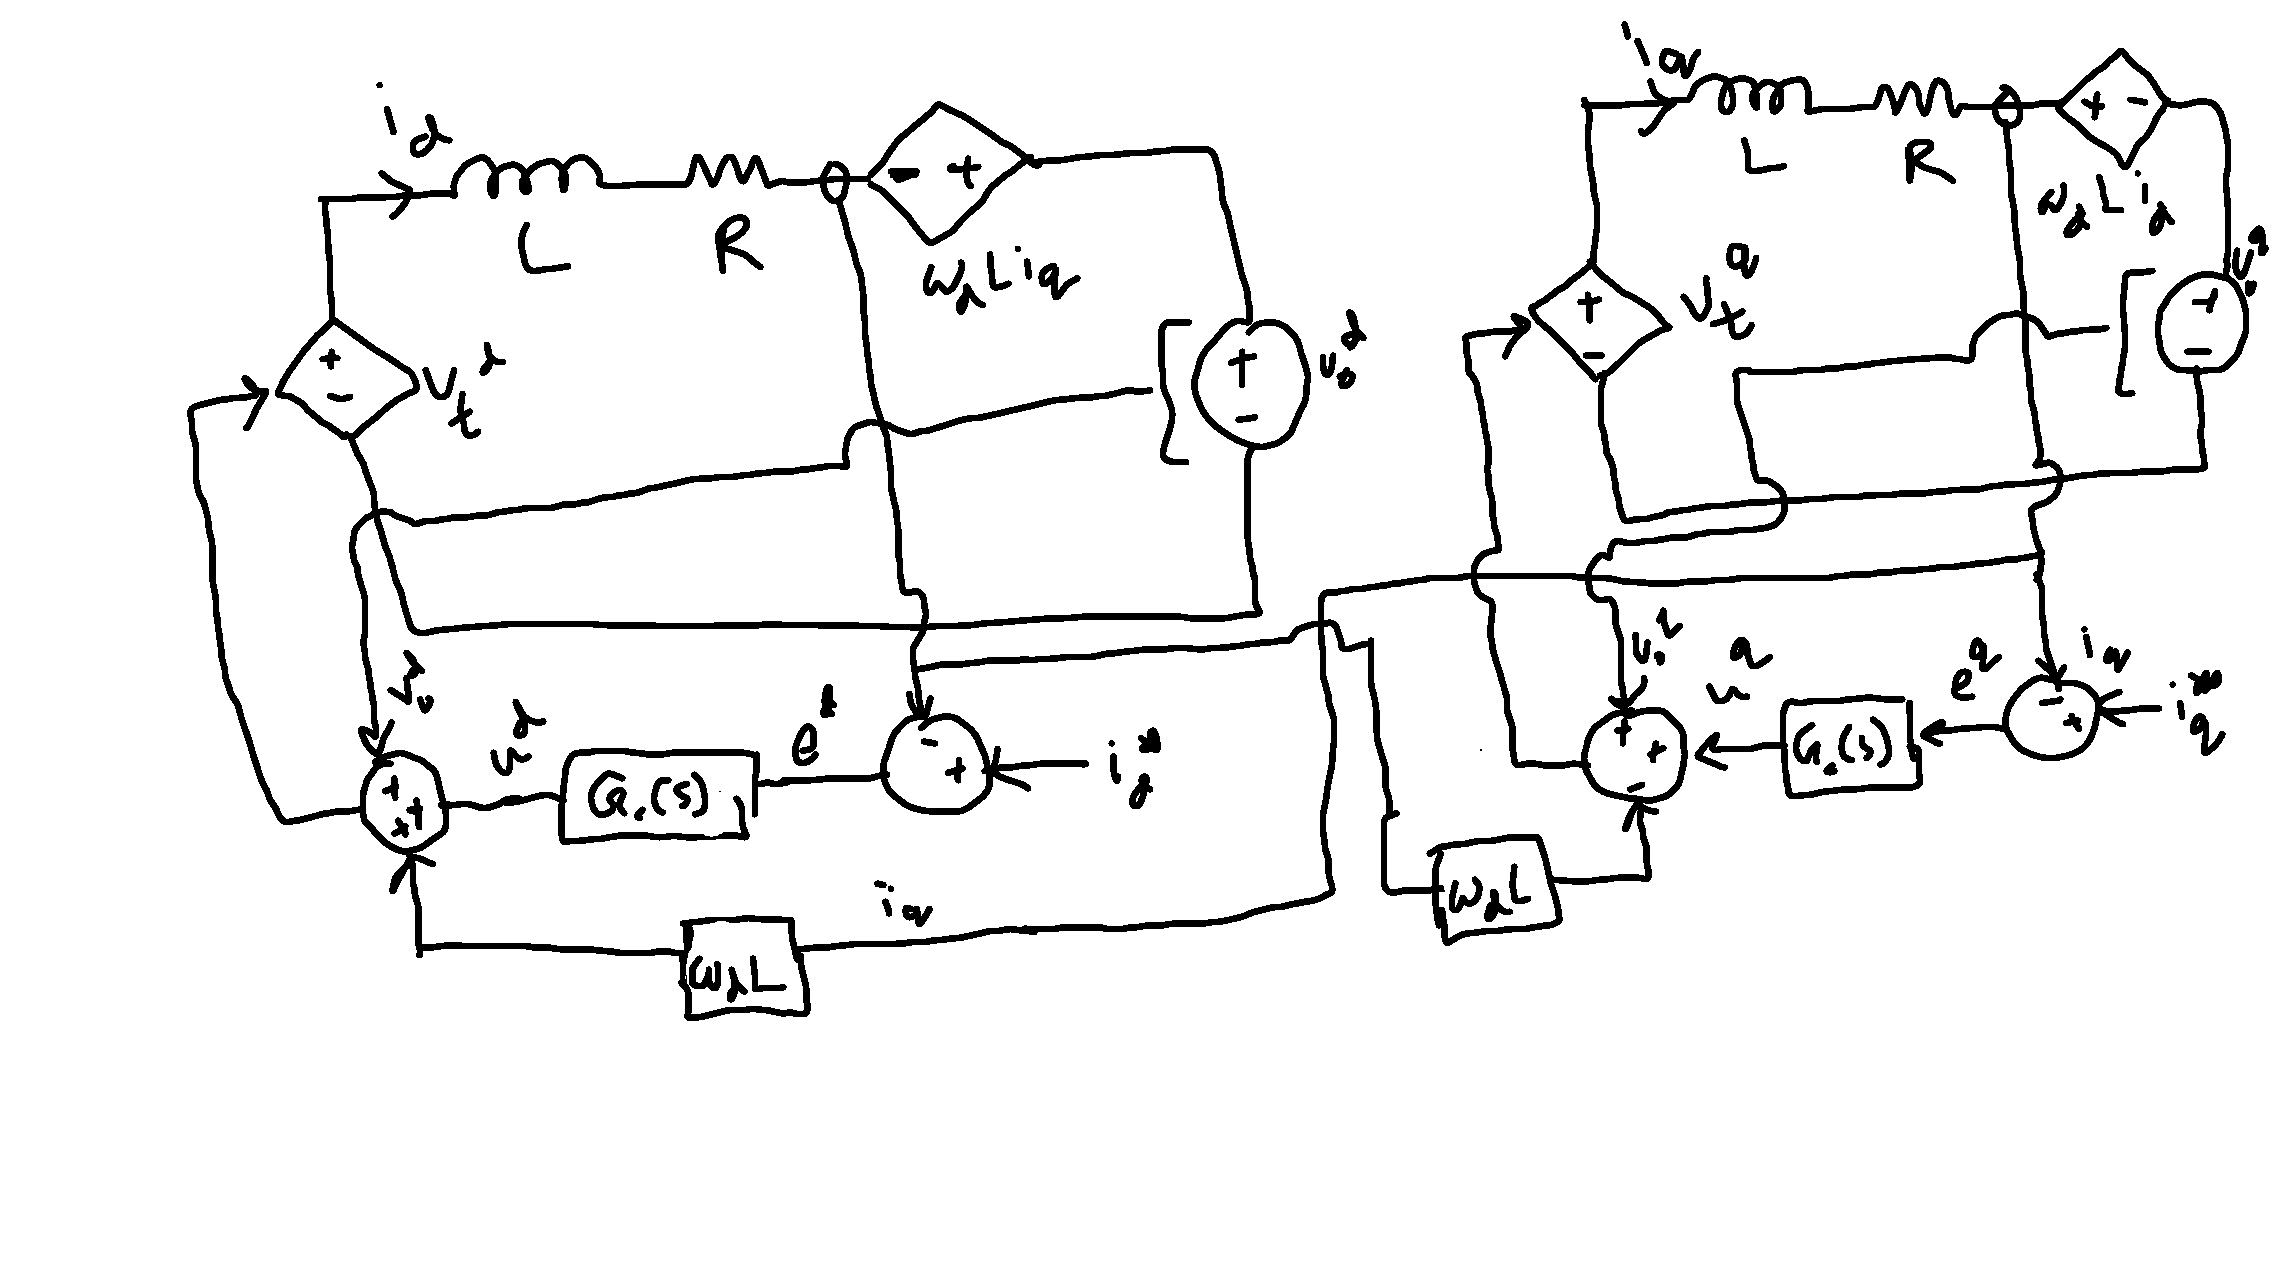
\includegraphics[scale=0.4,trim={2cm 4cm 0cm 0cm},clip]{q4_block_dia.pdf}
	\caption{Q4: Inverter feedback control block diagram}
	\label{fig:q4_block_dia}
\end{figure}
%----------------------------------------------------------------------------------------
%	SOLUTION 4.ii
%----------------------------------------------------------------------------------------
\subsection*{Problem 4.ii}
To derive the closed-loop transfer functions $\frac{i_{dq}(s)}{i_{dq}^*(s)}$, we need to ignore the cross-coupling terms and $v_{dc}$ in Fig.~3 (in the question). Then we can get the following the block diagram for $i_d(s)$ (similar diagram for $i_q(s)$ too) as shown in Fig.~\ref{fig:q4_tf}:
%%%%%%%%%%%%%%%%%%%%%%% TRANSFER FUNCTION %%%%%%%%%%%%%%%%%%%%%
\begin{figure}[!h]
	\centering
	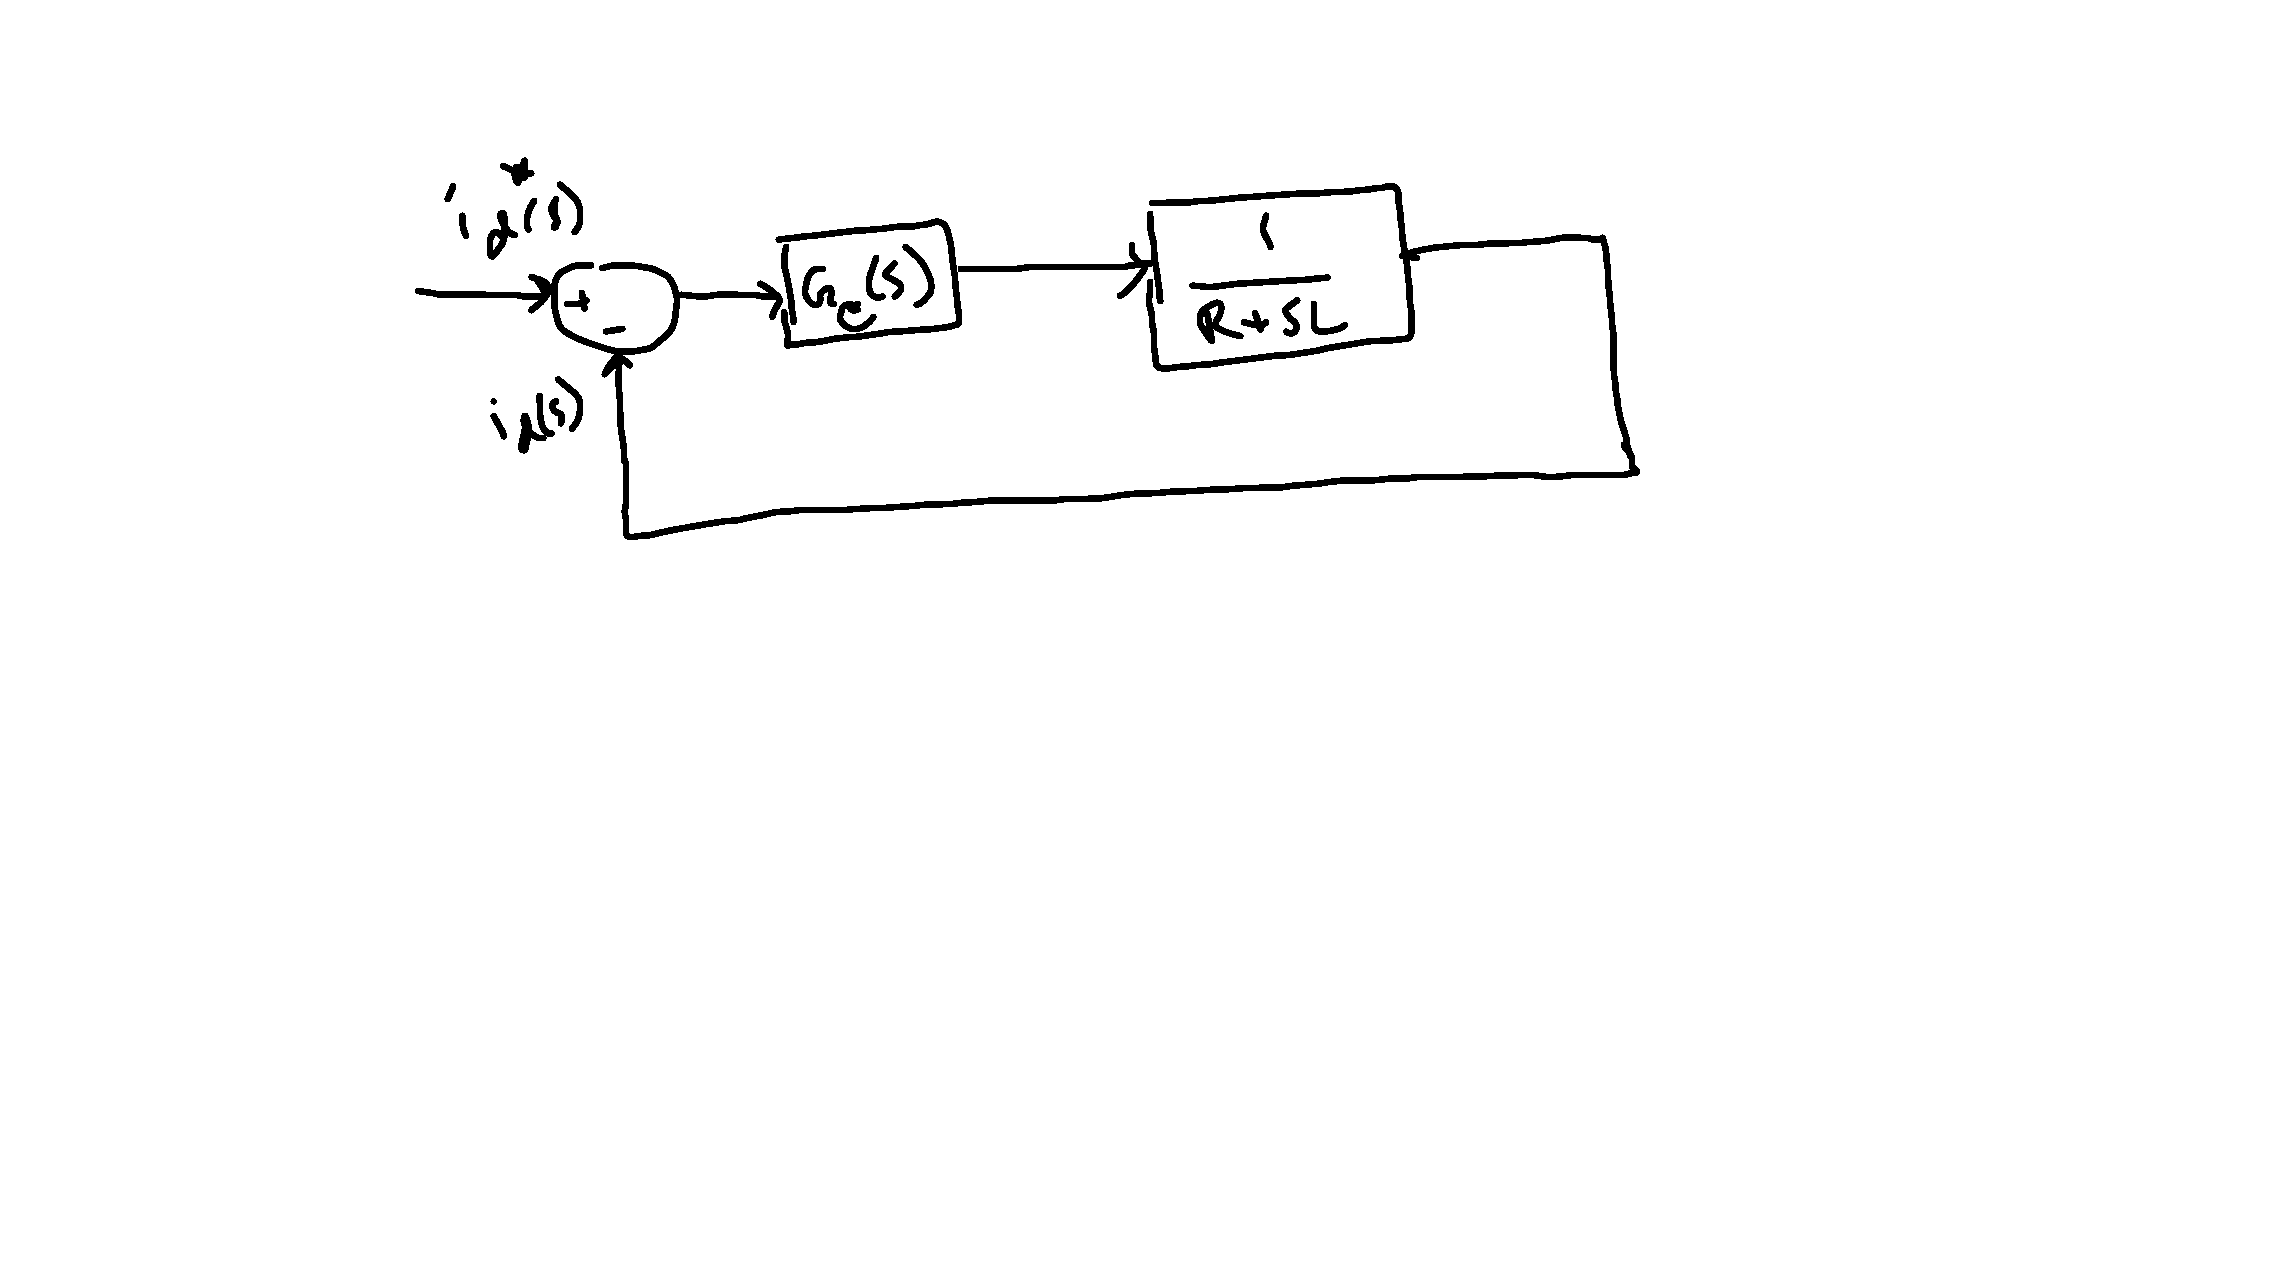
\includegraphics[scale=0.4,trim={2cm 12cm 0cm 0cm},clip]{q4_tf.pdf}
	\caption{Q4: Block diagram to derive current transfer function}
	\label{fig:q4_tf}
\end{figure}

Considering $G_c(s)=(k_p+k_i/s)$, we can derive the transfer function as follows:
\begin{align}\label{eq:q4_tf}
	H(s) &= \frac{i_d(s)}{i_d^*(s)} \nonumber\\
	&= \frac{G_c(s)/(R+sL)}{1+G_c/(R+sL)} \nonumber\\
	&= \frac{G_c(s)}{(R+sL)+G_c(s)} \nonumber\\
	&= \frac{k_p+k_i/s}{(k_p+k_i/s)+(R+sL)}.
\end{align}
%----------------------------------------------------------------------------------------
%	SOLUTION 4.iii
%----------------------------------------------------------------------------------------
\subsection*{Problem 4.iii}
From Eq.~\ref{eq:q4_tf}, we get,
\begin{align}\label{eq:q4_iii_a}
	H(s) &= \frac{sk_p+k_i}{s^2L+s(R+k_p)+k_i} \nonumber\\
	&= \frac{1}{\frac{s^2L}{sk_p+k_i}+\frac{s(R+k_p)}{sk_p+k_i}+\frac{k_i}{sk_p+k_i}}
\end{align}
Equating denominator of Eq.~\ref{eq:q4_iii_a} with that of desired transfer function $\frac{1}{1+\tau s}$, we get:
\begin{align*}
	&\frac{s^2L}{sk_p+k_i}+\frac{s(R+k_p)}{sk_p+k_i}+\frac{k_i}{sk_p+k_i} = (1+\tau s)\\
	\implies & s^2L+s(R+k_p)+k_i = s^2 \tau k_p + s(k_p+\tau k_i)+k_i.
\end{align*}
Equating corresponding coefficients of $s$, we get:
\begin{align*}
	L &= \tau k_p \implies \tau = \frac{L}{k_p}\\
	R+k_p &= k_p+\tau k_i \implies \tau = \frac{R}{k_i}.
\end{align*}
Therefore,
\begin{align*}
	&\frac{L}{k_p} = \frac{R}{k_i}\\
	\implies & \frac{L}{R} = \frac{k_p}{k_i}.
\end{align*}
Similarly, we can prove the \textit{only if} part as follows.\\
Let, $\frac{L}{R}=\frac{k_p}{k_i}=c$. Also denote $\tau \coloneqq \frac{R}{k_i}$. Then $\tau = \frac{L}{k_p}$ also. From Eq.~\ref{eq:q4_tf},
\begin{align*}
	H(s) &= \frac{k_p+k_i/s}{(k_p+k_i/s)+(R+sL)}\\
	&= \frac{1}{1+\frac{R+sL}{k_p+k_i/s}}\\
	&= \frac{1}{1+\frac{(R/k_i)+s(L/k_i)}{(k_p/k_i)+(1/s)}}\\
	&= \frac{1}{1+\frac{\tau+s\frac{L}{k_p}\frac{k_p}{k_i}}{c+(1/s)}}\\
	&= \frac{1}{1+\frac{\tau + sc\frac{L}{k_p}}{c+(1/s)}}\\
	&= \frac{1}{1+\frac{s\tau+s^2c\tau}{sc+1}}\\
	&= \frac{1}{1+\tau s}.
\end{align*}

    %%----------------------------------------------------------------------------------------
%	SOLUTION 5
%----------------------------------------------------------------------------------------
\subsection*{Problem 5}
It is given that the wind power random variable $V$ follows uniform distribution as follows
\begin{align*}
	V \sim U(5,20).
\end{align*}
Therefore the PDF and CDF is given by
\begin{align*}
	f_V(v) &= \begin{cases}
		\frac{1}{15},\ v \in [5,20]\\
		0,\ \text{otherwise}
	\end{cases}\\
	F_V(v) &= \begin{cases}
		0,\ v < 5,\\
		\frac{v-5}{15},\ v \in [5,20],\\
		1,\ v > 20.
	\end{cases}
\end{align*}
Now, it is given that
\begin{align*}
	V_c &= 0\\
	V_r &= 5\\
	V_F &= 15\\
	P_{rated} &= 1000 \text{ W}.
\end{align*}
Therefore,
\begin{align*}
	P(v\geq 5) &= 1-F_V(5) = 1\\
	P(v \geq 15) &= 1-F_V(15) = 0.33.
\end{align*}
It is not clear if the question asks for annual energy yield at rated power. I assume that the question asks for annual energy yield at rated power. Therefore, annual energy that the wind turbine would generate is
\begin{align*}
	8670(1-0.33)(1000) = 5.87\times 10^6 \text{ W-h}.
\end{align*}
    %\input{problem_2}
    %\input{solution_2}
\end{document}